\documentclass[a4paper,12pt]{book}
\usepackage{graphicx}
\usepackage{tabularx}
\usepackage{a4wide}
%\usepackage[bookmarks=false,breaklinks=true,pdfstartview=Fit]{hyperref}
\usepackage{amsfonts}
\usepackage{amsmath}
%\usepackage{listings}
% \usepackage{color}
\usepackage[usenames,dvipsnames]{color}
\usepackage{html}
%\usepackage{hyperref}
\usepackage{verbatim}

% \#c4ebff;

\begin{htmlonly}
\newcommand{\codebegin}{
\begin{rawhtml}
<div style="color: black; background-color: \#a9b8cb;  border-style: dotted; border-width: 1px;" >
\end{rawhtml}
}
\newcommand{\codeend}{
\begin{rawhtml}
</div>
\end{rawhtml}
}
\end{htmlonly}

%begin{latexonly}
\newcommand{\codebegin}{

}
\newcommand{\codeend}{

}
%end{latexonly}

\author{Joel Andersson \and Attila Kozma \and Joris Gillis \and Moritz Diehl}
\title{CasADi Users' Guide {\color{red}(WORKING COPY)}}
\begin{document}
%\htmlinfo*
%\sffamily
\titlepage
\maketitle
%\clearpage
\begin{latexonly}
\tableofcontents
\end{latexonly}
\clearpage

\chapter{Introduction}
{\color{red}Warning: The users' guide is not finished. This is only a working copy.}
This document gives a brief tutorial on the CasADi software package and on the interfaces that comes with it. We aim at
introducing the most important capabilities of what CasADi can do. Our fundamental motivation is to provide open-source
software for people working with numerical optimization, dynamic system simulation and optimal control.

Our explaination is mostly program code driven and provides little mathematical background knowledge. We assume that the reader already has a fair knowledge of either Python or C++, theory of differential equations and optimization theory. We will mainly use Python syntax in the discussion, which is the language we recommend using for getting familiar with CasADi, and try to point out the instances where the C++ or Octave syntax diverges from the Python syntax. To facilitate switching between the programming languages, we also list the major differences in chapter \ref{sec:syntax_differences}
The goal of this document is to make the reader familiar with the syntax of CasADi and provide easily available building blocks to build numerical optimization and dynamic optimization software.

After reading this users' guide, the reader should be able to formulate and manipulate symbolic expressions in CasADi, generate derivatives using automatic differentiation, to set up, solve and perform forward and adjoint sensitivity analysis for systems of ordinary differential equations (ODE) or differential-algebraic equations (DAE) as well as to solve nonlinear programming (NLP) problems and optimal control (OCP) problems.

\chapter{Installation}
In this section we introduce step by step the installation procedure of CasADi. First we detail what software packages need to
be installed in order to use CasADi.
\section{Software requirements}
CasADi consists of a symbolic core, which is strongly used by the interfaces that are shipped with it. Now we summarize
what the dependencies of each are. As a general rule you will always need a C++ compiler (tested with gcc 4.4.3) and
CMake (tested with version 2.8.2).
\begin{center}
\small
\begin{tabular}{|l|l|}
\hline
\textbf{Package/interface} & \textbf{Dependency}\\
\hline
CasADi core & None \\
\hline
CSparse interface & CSparse (comes with CasADi)\\
\hline
Ipopt interface & Ipopt\\
\hline
KNITRO interface & KNITRO\\
\hline
LAPACK interface & library with LAPACK api\\
\hline
LiftOpt interface & LiftOpt\\
\hline
Sundials interface & SUNDIALS \\
\hline
SuperLU interface & SuperLU, library with BLAS api\\
\hline
CasADi for python & SWIG \\
\hline
\end{tabular}
\end{center}
\section{Compilation}
First, you have to get CasADi from \htmladdnormallink{here}{http://www.casadi.org/} or check out the svn repository from SourceForge.
\par
\codebegin
\begin{verbatim}
svn co https://casadi.svn.sourceforge.net/svnroot/casadi/trunk casadi
\end{verbatim}
\codeend
Set the \texttt{CMAKE\_PREFIX\_PATH} to inform CMake where the dependecies are. 
For example if Sundials headers and libraries are installed under \texttt{\$HOME/local/}, then type
\par
\codebegin{
\begin{verbatim}
export CMAKE_PREFIX_PATH=$HOME/local/
\end{verbatim}
\codeend
\par
Go to directory of the source tree, create a directory called \texttt{build} where all compilation-related files will be created.
\par
\codebegin
\begin{verbatim}
cd casadi; mkdir build; cd build
\end{verbatim}
\codeend
Generate the \texttt{Makefile} by typing
\par
\codebegin
\begin{verbatim}
cmake ..
\end{verbatim}
\codeend
Check the output of CMake if the dependencies are correctly located. The interfaces without underlying libraries and headers won't be compiled.
Now compile the C++ libraries.
\par
\codebegin
\begin{verbatim}
make
\end{verbatim}
\codeend
If you wish to use the python interface you can compile it with the \texttt{python} target.
\par
\codebegin
\begin{verbatim}
make python
\end{verbatim}
\codeend

\chapter{Structure of CasADi}
{\color{red}THIS CHAPTER IS NOT UP-TO-DATE!}
In CasADi a very powerful symbolic abstraction of mathematical functions is implemented.
In this chapter we will learn how to create general functions out of our model equations, 
how to evaluate them and optionally their derivatives. We also give some instructional
examples to make it more easily understandable.

The backbone of CasADi is centered around some fundamental classes:
\begin{itemize}
 \item \texttt{SX} -- \emph{scalar symbolic type}
 \item \texttt{SXMatrix} -- \emph{sparse matrix with elements of type \texttt{SX}}
 \item \texttt{DMatrix}  -- \emph{same as \texttt{SXMatrix} but with elements of floating point type}
 \item \texttt{FX} and derived classes -- \emph{functions}
 \item \texttt{MX} -- \emph{matrix symbolic type}
\end{itemize}

\subsection{\texttt{SX} and \texttt{SXMatrix}}
The \texttt{SX} type is used to represent symbolic expressions made up by a sequence of unary and binary operations. It uses a syntax similar to a numeric type such as \texttt{float} in Python or a \texttt{double} in C/C++, but instead of calculating the expressions numerically, the \texttt{SX} will build up an expression. The type overloads most common operations and can also be used instead of container classes such as \texttt{numpy.array} in Python or \texttt{std::vector<>} in C++'s Standard Template Library (STL).

Though it is possible and somtimes benificial, we shall not work with the \texttt{SX} type directly in this tutorial. Instead we shall work with a \emph{sparse matrix type} called \texttt{SXMatrix}, whose elements are \texttt{SX} instances. \texttt{SXMatrix} uses an everything-is-a-matrix type syntax that should be familiar to Matlab users, which means that scalars can be represented as 1-by-1 matrices and vectors as $n$-by-1 matrices. To store its element, it uses a general sparse matrix format comparible to that used for sparse matrices in Matlab\footnote{To be more precise, the storage format used is \emph{compressed row storage}}.

To see how it works in practice, start an interactive Python shell (e.g. by typing \texttt{ipython} from a Linux terminal or inside a integrated development environment such as Spyder) and import CasADi using the command:\footnote{In C++, include the core header files through ''\texttt{\#include "casadi/casadi.hpp"}''. Classes and functions are defined in the namespace \texttt{CasADi}. In Octave, the CasADi module is imported by simply invoking \texttt{casadi}}

\begin{verbatim}
  from casadi import *
\end{verbatim}

Now create the variable \texttt{x} using the syntax (cf. the function \texttt{sym} in Matlab's Symbolic Toolbox)\footnote{In C++, since it is statically typed, you need to specify the return type, here \texttt{SXMatrix}. To find the return types for a CasADi function, use the C++ API docs on the website}:
\begin{verbatim}
  x = ssym("x")
\end{verbatim}
Note that the string passed is only the display name, not the identifier. Multiple variables can have the same name, but still be different. You can also create vectors or matrices of variables using by supplying additional arguments to \texttt{ssym}:
\begin{verbatim}
  y = ssym("y",5)   # A 5-by-1 matrix, i.e. a vector, with symbolic variables
  Z = ssym("Z",4,2) # A 4-by-2 matrix with symbolic variables
\end{verbatim}

Note that \texttt{ssym} is a function which returns an \texttt{SXMatrix} instance. When variables have been declared, expressions can now be formed in an intuitive way: 
\begin{verbatim}
  f = x**2 + 10  # "x**y" corresponds to "pow(x,y)" in C++
  f = sqrt(f)
  print "f = ", f
\end{verbatim}

You can also create \texttt{SXMatrix} instances \emph{without} any symbolic variables\footnote{In C++, class}:
\begin{verbatim}
 B1 = SXMatrix.zeros(4,5)  # a dense 4-by-5 empty matrix with all zeros
 B2 = SXMatrix.sparse(4,5) # a sparse 4-by-5 empty matrix with all zeros
 B3 = SXMatrix.ones(4,5)   # a dense 4-by-5 matrix filled with ones
 B4 = SXMatrix.eye(4)      # a sparse 4-by-4 matrix with ones on the diagonal
\end{verbatim}

Note the difference between a sparse matrix with \emph{structural} zeros and a dense matrix with \emph{actual} zeros. When printing an expression with structural zeros, these will be represented as $00$ to distinguish them from actual zeros $0$.

Elements are accessed and set using a bracket syntax, which also updates the sparsity pattern. Note that in C++ and Python (and thus also in CasADi) indices start with zero:
\begin{verbatim}
 print B1[0,0]   # print elements [0,0] (Python is zero-based!)
 print B2[-1,-1] # print the last element of the last row
 print B3[:,2]   # print all elements in the 3rd column
 B4[2:4,1]=[7,3] # set [2,1] to 7 and [3,1] to 3
\end{verbatim}

Remember to pass two arguments if you wish to access a matrix entry. If you call the same function using \emph{one} index, is interpreted as accesssing the (structural) nonzeros of the matrix:
\begin{verbatim}
 B4[:] = 5   # set all nonzeros to 5
 print B4[6] # error: there are only six nonzeros!
\end{verbatim}

There is a growing set of operations that can be performed with the \texttt{SXMatrix}, including:
\begin{itemize}
 \item Calculus: E.g. \verb|Jx = jacobian(f,x)|: Jacobian of expression \texttt{f} with respect to expression \texttt{x}, see also the \texttt{FX} member \emph{function} \texttt{jacobian} below.
 \item Algebra: E.g. \verb|x = solve(A,b)|: Can be used to give a symbolic expression for $x = A^{-1} \, b$.
\end{itemize}
It is typically uncomplicated to add new such functions whenever they appear in applications.

\subsection{\texttt{DMatrix}}
\texttt{DMatrix} is very similar to \texttt{SXMatrix} (in fact, they are just two template instantiations of the same C++ class \texttt{CasADi::Matrix<\,T\,>}), but with the difference that the nonzero elements are numerical values and not \texttt{SX} expressions. The syntax is also the same, except for functions such as \texttt{ssym} or \texttt{jacobian} which has no equivalent.

\texttt{DMatrix} is mainly used for storing matrices in CasADi and as inputs and outputs of functions. It is \emph{not} intended to be used for computationally intensive calculations. For this purpose, use \texttt{numpy} or \texttt{scipy} matrices in Python or an expression template based library such as \texttt{eigen}, \texttt{ublas} or \texttt{MTL} in C++. Conversion between the types is usually straightforward:
\begin{verbatim}
 C = 4*DMatrix.ones(2,3)
 C[:,2] = 5

 import numpy as NP
 C_numpy = NP.array(C)

 import scipy as SP
 C_scipy = SP.sparse.csr_matrix(C)
\end{verbatim}

More usage examples for \texttt{SX} can be found in the tutorials at \texttt{www.casadi.org}. For documentation of particular functions of this class (and others), find the ``C++ API docs'' on the website and search for information about \texttt{CasADi::Matrix<\,T\,>}.

\subsection{\texttt{FX} and derived classes}
CasADi contains a number of functions that all derive from the \texttt{FX} base class. This includes functions that are defined by a symbolic expression, ODE/DAE integrators, QP solvers, NLP solvers etc.

The usage skeleton of all these functions are:
\begin{verbatim}
# Call the constructor
f = ClassName(arguments)

# Set options
f.setOption("option_name",option_value)

# Initialize the function
f.init()

# Set inputs, forward and adjoint derivative seeds
f.setInput(value,input_index)
f.setFwdSeed(value,input_index)
f.setAdjSeed(value,output_index)

# Evaluate
f.evaluate(num_fwd_sensitivities, num_adj_sensitivities)

# Get outputs, forward and adjoint derivative sensitivities
f.getOutput(value,output_index)
f.getFwdSens(value,output_index)
f.getAdjSens(value,input_index)
\end{verbatim}

As an alternative to calling \texttt{getOutput}, \texttt{setFwdSeed} etc., you can also directly access the internal matrices (which are of type \texttt{DMatrix}). This can decrease overhead and shorten the code, but must be used with caution, since changing the \emph{structure} of these matrices can cause CasADi to crash.
\begin{verbatim}
print "output is ", f.output()
print "forward seed is ", f.fwdSeed()
\end{verbatim}

Note that all functions are multiple (sparse, matrix-valued) input, multiple (sparse, matrix-valued) output.

One of the \texttt{FX} derived classes is \texttt{SXFunction}, which defines a function given a symbolic expression. Its constructor is:
\begin{verbatim}
 f = SXFunction(list_of_inputs,list_of_outputs)
\end{verbatim}

\section{The \texttt{MX} symbolics}

Let us perform a simple operation using the \texttt{SXMatrix} above:
\begin{verbatim}
x = ssym("x",2,2)
y = ssym("y")
f = 3*x + y
print "f = ", f
\end{verbatim}

As you can see, the output of this operaton is the 2-by-2 matrix
\begin{verbatim}
[[((3*x_0_0)+y),  ((3*x_0_1)+y) ]
 [((3*x_1_0)+y),  ((3*x_1_1)+y) ]]
\end{verbatim}

Note how the multiplication and the addition were performed elementwise and new expressions (of type $SX$) were created for each entry of the result matrix.

We shall now introduce a second, more general \emph{matrix expression} type \texttt{MX}. The \texttt{MX} type allows, like \texttt{SX}, to build up expressions consisting of a sequence of elementary operations. But unlike \texttt{SX}, these elementary operations are not restricted to be scalar unary or binary operations ($\mathbb{R} \rightarrow \mathbb{R}$ or $\mathbb{R} \times \mathbb{R} \rightarrow \mathbb{R}$. Instead the elementary operations that are used to form \texttt{MX} expressions are allowed to be general \emph{multiple sparse-matrix valued} input, \emph{multiple sparse-matrix valued} output functions: $\mathbb{R}^{n_1 \times m_1} \times \ldots \times \mathbb{R}^{n_N \times m_N} \rightarrow \mathbb{R}^{p_1 \times q_1} \times \ldots \times \mathbb{R}^{p_M \times q_M}$. In particular, we allow \emph{calls} to functions of type \texttt{FX} (including calls to ODE integrators and \texttt{SXFunction} instances).

The syntax of \texttt{MX} is intended to mirror that of \texttt{SXMatrix}:
\begin{verbatim}
x = msym("x",2,2)
y = msym("y")
f = 3*x + y
print "f = ", f
\end{verbatim}

where \texttt{msym} has replaced \texttt{ssym}. The output of this expression is now simply:
\begin{verbatim}
((3*x)+y)
\end{verbatim}

Note that this operation required only 2 elementary operations (one multiplication and one addition) using \texttt{MX} symbolics, whereas the \texttt{SX} symbolics required 8 (2 for each element of the resulting matrix). \texttt{MX} is thus more economical when working with operations that are naturally vector or matrix valued. It is also much more general since we allow calls to arbitrary functions that cannot be expanded in terms of elementary operations (like a call to CVodes). %This extra generality, however, comes to the price of more overhead, and we shall 

\texttt{MX} supports getting and setting elements, using the same syntax as \texttt{SXMatrix}, but the way it is implemented is very different. Test, for example, to print the first column of a 2-by-2 symbolic variable:
\begin{verbatim}
x = msym("x",2,2)
print x[:,0] 
# Output: mapping(dense 2-by-1 matrix, dependencies: [x], nonzeros: [0,2])
\end{verbatim}

The output should be understood as a (linear) mapping from nonzeros 0 and 2 of the expression \texttt{x} to a new expression of dimension 2-by-1.

Similar outputs can be expected when trying to set elements:
\begin{verbatim}
x = msym("x",2)
A = MX.sparse(2,2)
A[0,0] = x[0]
A[1,1] = x[0]+x[1]
print A
# Output: mapping(diagonal 2-by-2 matrix, dependencies: [x,(x[0]+x[1])], \
#                 nonzeros: [0(0),0(1)]
\end{verbatim}
This time expression \texttt{A} becomes a mapping from \texttt{x} to a sparse 2-by-2 matrix. The interpretation of the cryptic output is that \texttt{A} is a linear mapping from $x$ and $x[0]+x[1]$ onto the diagonal of a (sparse) 2-by-2 matrix. The first nonzero of this mapping is the 0th nonzero of the 0th dependency ($x$) and the second nonzero is the 0th nonzero of the first dependency ($x[0]+x[1]$). 

Linear mappings, of the type you have seen here, is also the the result of several other operations that you might perform on an expression, including (but not limited to) matrix transposes, horizontal and vertical concatenations, resizings and reshapings.

This output tend to become quite hard to understand. An alternative (but not always better) way is to represent the function is as a graph:

\begin{minipage}[t]{0.45\textwidth}
\texttt{from casadi import tools} \\
\texttt{tools.dotdraw(A)} \\
\end{minipage}
\begin{minipage}[t]{0.45\textwidth}
\begin{center}
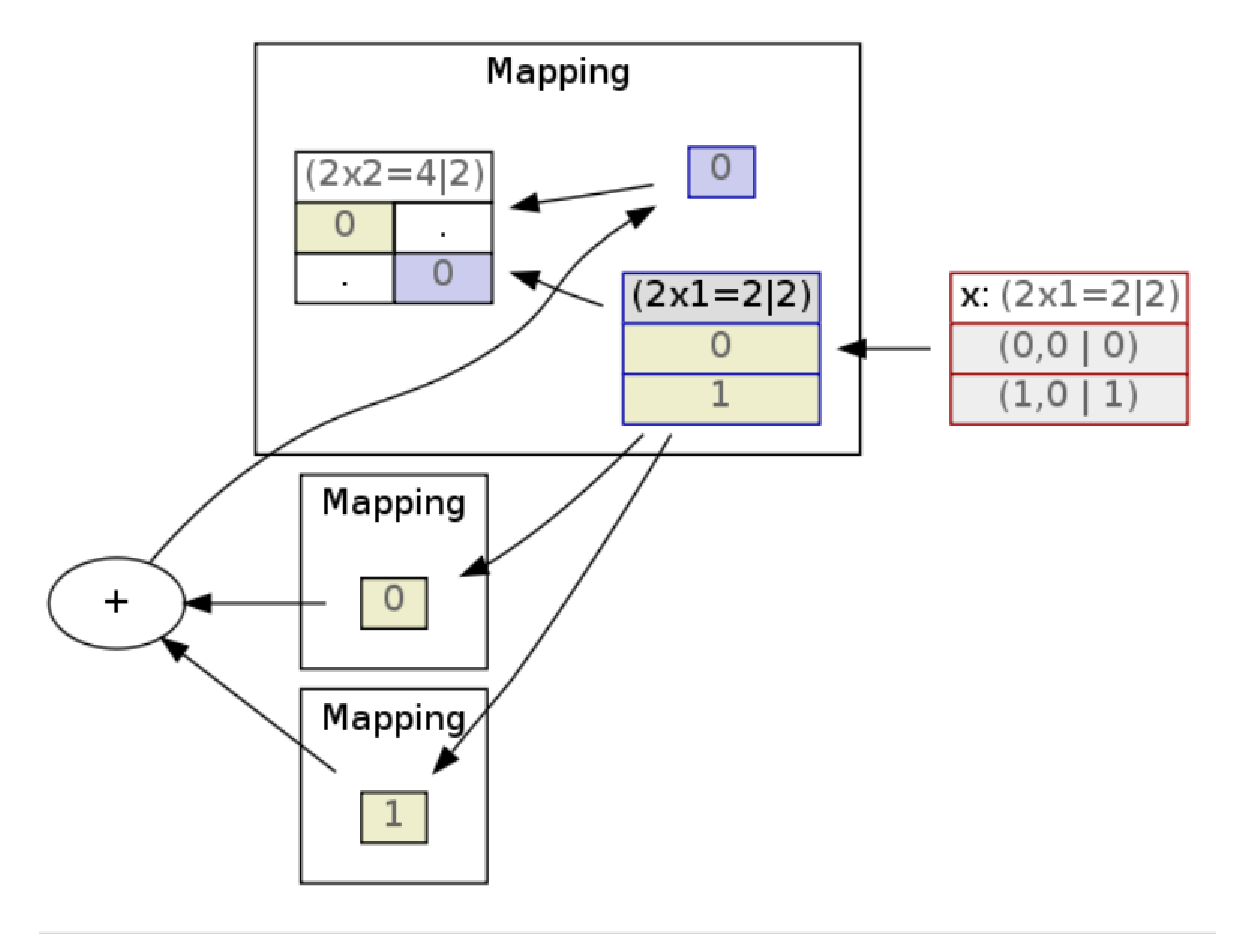
\includegraphics[width=\textwidth]{mxdraw}
\end{center}
\end{minipage}

Using this feature, which is still under development, requires that you have installed the Python package \emph{pydot}. We actively work on getting the expressions more easier to grasp.

\texttt{MX} expressions may contain calls to CasADi functions. To embed a call to an \texttt{FX}-derived function (e.g. \texttt{SXFunction} or \texttt{CVodesIntegrator}, see Section \ref{chapter:integrators}), you use the syntax:
\begin{verbatim}
[y1,y2,...,yn] = f.call([x1,x2,...,xn])
\end{verbatim}

Remember to put the brackets around the output even if the function only has a single output.

Expressions formulated using \texttt{MX} expressions can be used to formulate functions of type \texttt{MXFunction}:
\begin{verbatim}
 f = MXFunction(list_of_inputs,list_of_outputs)
\end{verbatim}

\section{Mixing \texttt{SX} and \texttt{MX}}
You can \emph{not} multiply an \texttt{SXMatrix} with a \texttt{MX}, or perform any other operation to mix the two in the same expression graph. You can, however, as mentioned above, include calls to an \texttt{SXFunction} in an \texttt{MX} graph. This is often a good idea since \texttt{SXFunction} is several times faster than \texttt{MXFunction} when dealing with small to medium size expressions (up to some thousands of variables). It is also much more stable and contains fewer bugs. 

The \texttt{SX} expressions is thus intended to be used for low level operations (for example the DAE right hand side), whereas the \texttt{MX} expressions act as a glue and enables the formulation of e.g. the constraint function of an NLP (which might contain calls to ODE/DAE integrators, or might simply be too large to expand as one big expression).

An \texttt{MXFunction} which only contains built-in operations (e.g. +, *, linear mappings, matrix multiplications and calls to \texttt{SXFunction} instances, can be converted into an \texttt{SXFunction} using the syntax:
\begin{verbatim}
 sx_function = SXFunction(mx_function)
\end{verbatim}

This might speed up the calculations significantly, but might also cause extra memory overhead.


\section{Symbolic expressions}
{\color{red}THIS SECTION AND THE REMAINDER OF THIS CHAPTER IS NOT UP-TO-DATE!}
Normally, mathematical expressions represent operations between variables and parameters.
In order to build up our models, we need to have a computer-based abstraction of these. In CasADi
the \texttt{\htmladdnormallink{SX}{http://casadi.sourceforge.net/api/html/d2/db3/classCasADi_1_1SX.html}} class provides us exactly these building blocks. We create a simple expression:
\par
\codebegin
\begin{verbatim}
     1  #include "casadi/sx/sx.hpp"
     2  using namespace CasADi;
     3  int main(int argc, char* argv[]){
     4     SX x("x");
     5     SX expr;
     6     cout << "x: " << x << endl;
     7     cout << "expr: " << expr << endl;
     8     expr = 3.0 * x + pow(x, 2) - sin(x);
     9     cout << "expr: " << expr << endl;
    10     SX y("y");
    11     expr += y / 2 / x;
    12     cout << "expr: " << expr << endl;
    13  }
\end{verbatim}
\codeend
And the output is
\par
\codebegin
\begin{verbatim}
   x: x
   expr: nan
   expr: (((3*x)+(x*x))-sin(x))
   expr: ((((3*x)+(x*x))-sin(x))+((y/2)/x))
\end{verbatim}
\codeend
On the 1st line we include the header file containing the \texttt{SX} class, on the 4th the \texttt{x} object
is created and from here on the string \texttt{"x"} is assigned to this variable. We can also create 
\texttt{SX} objects by invoking the default constructor (as we do on line 5), although this variable is not initialized to any symbolic
expression at this time. The \texttt{expr} object is initialized on the 8th line, while from the 10th line on we extend our expression
with a \texttt{y} variable. One can always check whether an expression is correct by simply printing it to the standard output.\\
With the use of \texttt{SX} objects and the \texttt{+ - * / += -= *= /= exp log sqrt sin pow} etc. operations we can build up a
wide range of mathemetical expressions.
\par
We can also create a vector of expressions if needed, although each element must be initialized that may be
carried out by the \texttt{make\_symbolic} function. Now we demonstrate how this works.
\par
\codebegin
\begin{verbatim}
     1  #include "casadi/sx/sx.hpp"
     2  #include "casadi/sx/sx_tools.hpp"
     3  
     4  ...
     5  vector<SX> z(10);
     6  make_symbolic(z.begin(), z.end(), "z");
     7  cout << "z[4]: " << z[4] << endl;
     8  ...
\end{verbatim}
\codeend
After invoking \texttt{make\_symbolic} on the 6th line the elements of \texttt{z} are assigned to \texttt{z\_0, z\_1, $\dots$} and can be used later on in modelling.
\section{Functions}
{\color{red}THIS SECTION AND THE REMAINDER OF THIS CHAPTER IS NOT UP-TO-DATE!}
Now that we can build up mathematical expressions we would like to evaluate them symbolically or numerically. We will see how this can be
done with the \texttt{SXFunction} object, which can represent mathematical functions that has prototype
 $\mathbb{R} \rightarrow \mathbb{R}$, $\mathbb{R}^n \rightarrow \mathbb{R}$,
$\mathbb{R}^n \rightarrow \mathbb{R}^m $ or $\mathbb{R}^{n_1 \times n_2} \rightarrow \mathbb{R}^{m_1 \times m_2}$.
In the constructor of \texttt{\htmladdnormallink{SXFunction}{http://casadi.sourceforge.net/api/html/d2/d58/classCasADi_1_1SXFunction.html}} one has to give two arguments. The first argument should contain all the variables
that the function will depend on, and the second argument stores the function definition itself. The data type of the arguments may be various
depending on the prototype of the function that is to be represented. Let's see some examples.
\subsection*{Numerical evaluation}
Most often we would like to compute the value of a function in a certain point. In this subsection we will learn how to do that
 in case of different function prototypes.
First we create and evaluate a simple scalar-scalar function numerically.
\par
\codebegin
\begin{verbatim}
     1  #include "casadi/sx/sx.hpp"
     2  ...
     3  SX x("x");
     4  SX f_expr = x * x - 3 * x + 2;
     5  SXFunction f(x, f_expr);
     6  f.init();
     7  double d = 10.0;
     8  f.setInput(d);
     9  f.evaluate();
    10  cout << "Function value in x = " << d << " : " << f.output() << "\n";
\end{verbatim}
\codeend
On the 4th line we create the expression that will represent our function. The \texttt{SXFunction}
object is created on the 5th line with the variable \texttt{x} and the \texttt{f\_expr} object.
Before passing any input to the function, we have to initialize it on line 6. Then we set the input
of the function, evaluate it and finally print the result.
\par\noindent
Now we create a vector-scalar function that calculates the 2-norm of its argument.
\par
\codebegin
\begin{verbatim}
     1  vector<SX> x(4);
     2  make_symbolic(x.begin(), x.end(), "x");
     3  SX f_expr = 0;
     4  for(int i = 0; i < x.size(); ++i){
     5     f_expr += x[i] * x[i];
     6  }
     7  f_expr = sqrt(f_expr);
     8  SXFunction f(x, f_expr);
     9  f.init();
    10  vector<double> d(x.size());
    11  fill(d.begin(), d.end(), 3);
    12  f.setInput(d);
    13  f.evaluate();
    14  cout << "Function value: " << f.output() << "\n";
\end{verbatim}
\codeend
The principle is exactly the same, the only difference is that now we pass a \texttt{std::vector<SX>} in the first argument
on line 8 and we provide a \texttt{std::vector<double>} as an input on line 12.
\par\noindent
Now we define and evaluate a vector-vector function.
\par 
\codebegin
\begin{verbatim}
     1  vector<SX> x(3);
     2  make_symbolic(x.begin(), x.end(), "x");
     3  vector<SX> f_expr(2);
     4  fill(f_expr.begin(), f_expr.end(), 0);
     5  f_expr[0] = x[0] + 2 * x[1];
     6  f_expr[1] = x[1] + 4 * exp(x[2]);
     7  SXFunction f(x, f_expr);
     8  f.init();
     9  vector<double> d(3);
    10  fill(d.begin(), d.end(), 2);
    11  f.setInput(d);
    12  f.evaluate();
    13  vector<double> value = f.output();
    14  cout << "[" << value.size() << "](";
    15  for(int i = 0; i < value.size(); ++i){
    16     cout << value[i] << ",";
    17  }
    18  cout << "\b)\n";
\end{verbatim}
\codeend
This time both arguments of the constructor on line 7 are \texttt{std::vector<SX>}
 and the return value of the
 \texttt{output()} member function is a \texttt{std::vector<double>} (line 13).
\par\noindent
As the last example let's see a piece of code, where the function depends on a  \texttt{std::vector<std::vector<SX> >}. 
Note that this covers the case when our function depends on a matrix.
\par
\codebegin
\begin{verbatim}
     1  vector<vector<SX> > variables;
     2  vector<SX> x(3);
     3  make_symbolic(x.begin(), x.end(), "x");
     4  variables.push_back(x);
     5  vector<SX> y(2);
     6  make_symbolic(y.begin(), y.end(), "y");
     7  variables.push_back(y);
     8  vector<SX> f_expr(2);
     9  f_expr[0] = x[0] + x[2] - sin(y[0]);
    10  f_expr[1] = cos(x[1] - y[1]);
    11  SXFunction f(variables, f_expr);
    12  f.init();
    13  vector<double> d0(3);
    14  fill(d0.begin(), d0.end(), 6.0);
    15  vector<double> d1(2);
    16  fill(d1.begin(), d1.end(), 3.0);
    17  f.setInput(d0, 0);
    18  f.setInput(d1, 1);
    19  f.evaluate();
    20  vector<double> value = f.output();
    21  cout << "[" << value.size() << "](";
    22  for(int i = 0; i < value.size(); ++i){
    23     cout << value[i] << ",";
    24  }
    25  cout << "\b)\n";
\end{verbatim}
\codeend
In variable \texttt{variables} we collect vectors of \texttt{SX} objects. On line 17 and 18 you can notice
a new argument (which was always 0 until now) that addresses an input vector. In this example on the first coordinate
we have a 3 long vector, on the second we have a 2 long vector, which correspond to the function definition (line 11).
It is important to understand the concept of functions depending on matrices, because, as it will be shown later on (see
Chapter \ref{chapter:integrators} about integrators),
integrators are exactly of this type.
 \subsection*{Symbolic evaluation}
 \par\noindent
 One might also wish to replace certain variables in a symbolic expression with some other variables
  or with more complex expressions. This may be carried out easily by the use of symbolic evaluation, we use
  the \texttt{eval(...)} member function of the \texttt{SXFunction} class.
\par
\codebegin
\begin{verbatim}
     1  vector<SX> x(3);
     2  make_symbolic(x.begin(), x.end(), "x");
     3  vector<SX> f_expr(2);
     4  f_expr[0] = x[0] + 5 * x[1];
     5  f_expr[1] = x[0] + cos(x[2]);
     6  SXFunction f(x, f_expr);
     7  f.init();
     8  vector<SX> y = x;
     9  y[0] = x[1] + pow(x[2], 3);
    10  vector<SX> f_expr_subs = f.eval(y);
    11  cout << f_expr[0] << " --> " << f_expr_subs[0] << endl;
    12  cout << f_expr[1] << " --> " << f_expr_subs[1] << endl;
\end{verbatim}
\codeend
First we create a function depending on the vector \texttt{x} (line 1 \-- 7), then we create a vector of \texttt{SX} objects, whose
size correspond to the function definition and we modify the first element by an arbitrary expression (line 9). As a result we get
back the function expression in which the substitution has already been committed.
\chapter{Automatic differentiation\label{chapter:ad}}
The most important functionality of CasADi is \emph{automatic differentiation} or AD. CasADi contains a total of 8 different AD algorithms that are suitable in different situations.

Given a function $\mathbf{R}^N \rightarrow \mathbf{R}^M$:
\begin{equation}
 y = f(x)
\end{equation}

forward directional derivatives (Jacobian-times-vector products) can be calculated by giving a \emph{seed} in that direction:
\begin{equation}
 y_{\text{fsens}} = \frac{\partial f}{\partial x} \, x_{\text{fseed}}
\end{equation}

Jacobian-transposed-times-vector products can be calculated in a similar way, using adjoint mode AD:
\begin{equation}
 x_{\text{asens}} = \left(\frac{\partial f}{\partial x}\right)^{\text{T}} \, y_{\text{aseed}}
\end{equation}

In CasADi, forward/adjoint seeds are set together with the function inputs and forward/adjoint sensitivities (or directional derivatives) are collected together with the outputs. Multiple forward and/or adjoint derivative directions can be handled simultaneously, that is you can simultaneously multiply the Jacobian from the left or right with multiple vectors. The number of vectors are passed as arguemnts to \texttt{f.evaluate(num\_fwd\_sensitivities, num\_adj\_sensitivities)}. In this turorial we shall restrict ourselves to at most one forward and one adjoint derivative direction, meaning that \texttt{num\_fwd\_sensitivities} and \texttt{num\_adj\_sensitivities} will either be 0 or 1.

CasADi is also able to generate complete, \emph{sparse} Jacobians efficiently by calling the \texttt{jacobian} member function. The algorithm it will use for this depends on the particular class\footnote{For \emph{SXFunction}, the default algorithm is to first determine the sparsity pattern, then use a graph coloring algorithm to determine which rows or columns can be calculated simultaneously, performing the AD algorithm symbolically and then assemble a new \emph{SXFunction} corresponding the the Jacobian}.
\begin{verbatim}
 Jf = f.jacobian(0,0) # function corresponding to the jacobian
                      # of the 0-th output w.r.t. the 0-th input
\end{verbatim}


\section{Calculating derivatives}
{\color{red}THIS SECTION AND THE REMAINDER OF THIS CHAPTER IS NOT UP-TO-DATE!}
In this section we will learn how to calculate first-order derivatives of general functions. Within CasADi derivatives of general
functions may be calculated in two ways. First, the derivatives are calculated numerically based on automatic differentiation,
 which has two modes forward and backward. Second, knowing the symbolic representation of the functions one may differentiate
 symbolically.

\subsection*{Forward differentiation}
 In the forward mode one can calculate the directional derivative
$J p$, where $J$ is the Jacobian of a $f: \mathbb{R}^n \rightarrow \mathbb{R}^m$ and $p \in \mathbb{R}^m$ is the direction.
In the following code we calculate the full Jacobian providing multiple directions.
\par
\codebegin
\begin{verbatim}
     1  vector<SX> x(3);
     2  make_symbolic(x.begin(), x.end(), "x");
     3  vector<SX> f_expr(2);
     4  f_expr[0] = x[0] + 5 * x[1];
     5  f_expr[1] = x[0] + cos(x[2]);
     6  SXFunction f(x, f_expr);
     7  f.setOption("number_of_fwd_dir", (int)x.size());
     8  f.init();
     9  vector<double> d(x.size());
    10  fill(d.begin(), d.end(), 4.0);
    11  f.setInput(d);
    12  vector<double> fwd_seed(x.size());
    13  fill(fwd_seed.begin(), fwd_seed.end(), 0);
    14  for(int i = 0; i < x.size(); ++i){
    15     fwd_seed[i] = 1;
    16     f.setFwdSeed(fwd_seed, 0, i);
    17     fwd_seed[i] = 0;
    18  }
    19  f.evaluate(1, 0);
    20  cout << "Function value: " << f.output() << endl;
    21  vector<double> jacobian_column;
    22  for(int i = 0; i < x.size(); ++i){
    23     jacobian_column = f.fwdSens(0, i);
    24     cout << "[" << jacobian_column.size() << "](";
    25     for(int j = 0; j < jacobian_column.size(); ++j){
    26        cout << jacobian_column[j] << ",";
    27     }
    28     cout << "\b)\n";
    29  }
\end{verbatim}
\codeend
The first new thing is on line 7, we set an option called \texttt{number\_of\_fwd\_dir} to the number
of the forward directions in which we would like to differentiate. On line 16 we are inside a for loop
and we provide the directions; now only columns of the identity matrix. The way of evaluation is also
slightly different (linr 19), so far we haven't given any arguments. The first argument indicates that we would like
forward derivatives to be evaluated as well as function evaluation, the second is just the same,
 but with adjoint derivatives. We can collect our
directional derivatives by the \texttt{fwdSens(...)} member function (line 23). Note that the first argument addresses
the the matrix input. Since we have only vector input now, this is always zero.
\subsection*{Backward (adjoint) differentiation}
In this mode of derivative calculation one can calculate $J^T p$. Mutiple directions are not yet supported by CasADi.
The code is as follows:
\par
\codebegin
\begin{verbatim}
     1  vector<SX> x(3);
     2  make_symbolic(x.begin(), x.end(), "x");
     3  vector<SX> f_expr(2);
     4  f_expr[0] = x[0] + 5 * x[1];
     5  f_expr[1] = x[0] + cos(x[2]);
     6  SXFunction f(x, f_expr);
     7  f.setOption("number_of_adj_dir", 1);
     8  f.init();
     9  vector<double> d(x.size());
    10  fill(d.begin(), d.end(), 4.0);
    11  f.setInput(d);
    12  vector<double> adj_seed(f_expr.size());
    13  fill(adj_seed.begin(), adj_seed.end(), 1);
    14  f.setAdjSeed(adj_seed, 0, 0);
    15  f.evaluate(0, 1);
    16  cout << "Function value: " << f.output() << endl;
    17  cout << "Adjoint derivative: " << f.adjSens(0, 0) << endl;
\end{verbatim}
\codeend
This time we set the option \texttt{number\_of\_adj\_dir} (greater than 1 throws an error) and we invoke \texttt{evaluate(0, 1)}.
The adjoint derivative we can access by the \texttt{adjSens(...)} method.
\par
\subsection*{Symbolic differentiation}
The second way one can differentiate is by symbolic manipulation. The result of this approach is nothing else than a
function symbolically representing the first derivative of the original function. The following example demonstrates this.
\par
\codebegin
\begin{verbatim}
     1  vector<SX> variables;
     2  vector<SX> x(3);
     3  make_symbolic(x, "x");
     4  variables = x;
     5  vector<SX> f_expr(2);
     6  f_expr[0] = x[0] + x[2] - sin(x[0]);
     7  f_expr[1] = cos(x[1] - x[2] * x[0]);
     8  SXFunction f(variables, f_expr);
     9  f.init();
    10  SXFunction f_der = f.jacobian();
    11  cout << "f: " << f.outputSX() << "\n"; 
    12  cout << "f_der: " << f_der.outputSX() << "\n";
    13  vector<double> d0(3);
    14  fill(d0.begin(), d0.end(), 6.0);
    15  f_der.init();
    16  f_der.setInput(d0);
    17  f_der.evaluate();
    18  cout << "Jacobian: " << f_der.output() << "\n"; 
\end{verbatim}
\codeend
The code is very self-explanatory, we create a vector-vector function (line 1-9) and invoke the \texttt{jacobian()} method, which
returns an \texttt{SXFunction} object. This object, since it's a function itself, can be evaluated and differentiated again.
This way we may calculate higher-order derivatives.


\chapter{ODE/DAE integration and sensitivity analysis\label{chapter:integrators}}
\section{ODE/DAE formulation}
The integrators interfaced with CasADi assumes a DAE residual function of the fully implicit form:
\begin{equation}
 f(t,x,p,\dot{x}) = 0
\end{equation}

Solvers for \emph{ordinary} differential equations will make the additional assumption that the structure of the function is:
\begin{equation}
 f_{\text{ode}}(t,x,p) - \dot{x} = 0
\end{equation}
the explicit equation for $\dot{x}$ can thus be retrieved by simply evaluating the DAE function with $\dot{x} = 0$.

It is important that the arguments of the function uses the order above, and for this reason, we strongly recommend users to work with a set of constants defining the required input and output schemes of the function. For the DAE residual function, these constants are \texttt{DAE\_NUM\_IN=4}, \texttt{DAE\_T=0}, \texttt{DAE\_Y=1}, \texttt{DAE\_P=2} and \texttt{DAE\_YDOT=3} for the inputs and \texttt{DAE\_NUM\_OUT=1} and \texttt{DAE\_RES=0} for the outputs.

An integrator in CasADi is a function that take the state at the initial time, guesses for the algebraic states and state derivatives (only important for DAEs) and evaluates the state vector at the final time. The time horizon is assumed to be fixed\footnote{for problems with free end time, you can always scale time by introducing an extra parameter and substitute $t$ for a dimensionless time variable that goes from 0 to 1} and can be set with the option:
\begin{verbatim}
 integrator.setOption("tf",integration_end_time)
\end{verbatim}

\section{Sundials integrators}
The Sundials suite contains the two popular integrators CVodes and IDAS for ODEs and DAEs respectively. These two integrators supports forward and adjoint sensitivities and when used via CasADi's Sundials interface, CasADi will automatically formulate the Jacobian information, which is needed by the backward differentiation formula (BDF) that CVodes and IDAS use. Also automatically formulated will be the forward and adjoint sensitivitiy equations. This means that the only information that the user needs to provide is the DAE residual function:
\begin{verbatim}
 integrator = CVodesIntegrator(f)   or  integrator = IdasIntegrator(f)
\end{verbatim}
for CVodes and IDAS respectively.

For a list of options for the integrators, as well as the input and output schemes of this \emph{function}, check the documentation directly from Python:
\begin{verbatim}
 CVodesIntegrator?
\end{verbatim}
or by consulting the online C++ API docs on the website.

\section{Sensitivity analysis}
From evaluation point of view, an integrator behaves just like the \texttt{SXFunction} introduced in the previous session. You set inputs, forward/adjoint seeds, evaluate and obtain the outputs and forward/adjoint sensitivities.

\section{The \texttt{Simulator} class}
As already mentioned, integrators in CasADi are functions that calculates the state at the final time. Often, however, a user is interested in obtaining the solution at multiple time points. This can often be done more efficiently than by repeatedly calling \texttt{integrator.evaluate()}. The easiest way to use this functionality is to use the \texttt{Simulator} class.

A \texttt{Simulator} can be created using the syntax:
\begin{verbatim}
  # Import numpy
  import numpy as NP

  # Allocate an integrator instance
  integrator = ...
  integrator.setOption("...",...)

  # Choose a time grid
  tgrid = NP.linspace(0,end_time,num_time_steps)

  # Create a simulator
  simulator = Simulator(integrator, time_grid)
\end{verbatim}

A \texttt{Simulator} can be used just like an integrator, and its input scheme is the same. Its output is now matrix valued, with the the columns corresponding to different time points. The class can also be used to evaluate a particular function of the state at a set of time points. See the API documentation for more information.

\section{Integration of explicit ODEs}
{\color{red}THIS SECTION AND THE REMAINDER OF THIS CHAPTER IS NOT UP-TO-DATE!}
In this section we will study how to use integrators and calculate sensitivites. Most of the things are already known from previous sections
since integrators transparently behave like functions. We are concerned with the following explicit ODE.
\begin{align}
\dot{x} &= f(x(t), p)\\
\dot{y} &= g(x(t), p)\\
x(0) &= x_0
\end{align}
In the following piece of code we show how easy it is to solve ODEs with quadratures.
\par
\codebegin
\begin{verbatim}
     1  SX t("t"); SX u("u"); SX s("s"); SX v("v"); SX m("m");
     2  vector<SX> ode(3);
     3  ode[0] = v;
     4  ode[1] = (u - 0.02 * v * v) / m;
     5  ode[2] = -0.01 * u * u;
     6  vector<SX> quad(2);
     7  quad[0] = s;
     8  quad[1] = 0.45 * m * v * v;
     9  vector<vector<SX> > ode_vars(3);
    10  ode_vars[0].push_back(t);
    11  ode_vars[1].push_back(s); ode_vars[1].push_back(v); ode_vars[1].push_back(m);
    12  ode_vars[2].push_back(u);
    13  SXFunction ode_func(ode_vars, ode);
    14  SXFunction quad_func(ode_vars, quad);
    15  CVodesIntegrator integrator(ode_func, quad_func);
    16  integrator.init();
    17  integrator.setInput(0.0, INTEGRATOR_T0);
    18  integrator.setInput(1.0, INTEGRATOR_TF);
    19  vector<double> x0(3 + 2);
    20  fill(x0.begin(), x0.end(), 0.0);
    21  x0[0] = 0; x0[1] = 1; x0[2] = 10;
    22  integrator.setInput(x0, INTEGRATOR_X0);
    23  vector<double> p(1);
    24  p[0] = 0.15;
    25  integrator.setInput(p, INTEGRATOR_P);
    26  integrator.evaluate();
    27  vector<double> xf = integrator.output(INTEGRATOR_XF);
    28  cout << "Solution of ODE: (";
    29     for(int j = 0; j < 3; ++j){
    30        cout << xf[j] << ",";
    31     }
    32     cout << "\b)\n";
    33  cout << "Solution of quadrature: (";
    34     for(int j = 3; j < 5; ++j){
    35        cout << xf[j] << ",";
    36     }
    37     cout << "\b)\n";
\end{verbatim}
\codeend
First of all we introduce a time variable (\texttt{t}), a control parameter (\texttt{u}) and three dynamic variables(\texttt{s, v, m}).
Their data type do not differ, but their use will give them different meaning. We build up our ODE equations (line 2-5) and quadrature formula
(line 6-8). Then we collect all our variables in a vector of vectors. In case of integrators one must respect the following rules regarding the
function variables. The first element
is a vector containing only the time variable (line 10). The second element is always the vector of all dynamic variables (line 11).
The third element contains the parameters (now we have only one control variable, line 12). Afterwards, we have to define two functions corresponding
to our ODE (line 13) and quadrature equations (line 14). Now everything is ready to instantiate the \texttt{CVodesIntegrator class}, which is an interface
to the CVODES algorithm. If we have no quadratures then we simply pass only the ODE equations (line 15). If we don't set any options a BDF method is used
to carry out integration. Later on we detail what options integrators and especially the \texttt{CVodesIntegrator} class has.
\par After initialization we set the time interval and initial value of the problem. We use the already known \texttt{setInput} method and the
\texttt{INTEGRATOR\_T0} and \texttt{INTEGRATOR\_TF} enum types to address the initial and final time (line 17-18). The initial value of the dynamic
variables is set by the use of \texttt{INTERGRATOR\_X0}. Note that CVODES handles quadratures by introducing dummy dynamic variables and thus the initial
value must have length of 3 + 2 = 5 in our example (line 19-22). The parameters (in our case \texttt{u}) should also be assigned a value, this may be done
using the \texttt{INTEGRATOR\_P} enum type (line 25).After evaluation we can access the solution of the ODE and quadratures by the \texttt{output} method
saying that we would like the value of the dynamic variables at the final time \texttt{INTEGRATOR\_XF} (see line 27).
%\subsection*{Evaluation of integrators}
\subsection*{Evaluation of forward and backward sensitivities}
As \texttt{CVodesIntegrator} is actually a special function, it is natural to expect first-order derivatives from it. Of course the underlying CVODES integrator must
provide sensitivities with respect to the initial value and the parameters used in the equations. We extend our previous source code and explain only the relevant parts.
\par
\codebegin
\begin{verbatim}
     1  CVodesIntegrator integrator(ode_func, quad_func);
     2  integrator.setOption("number_of_fwd_dir", 1);
     3  integrator.setOption("number_of_adj_dir", 1);
     4  integrator.init();
     5  integrator.setInput(0.0, INTEGRATOR_T0);
     6  integrator.setInput(1.0, INTEGRATOR_TF);
     7  vector<double> x0(3 + 2);
     8  fill(x0.begin(), x0.end(), 0.0);
     9  x0[0] = 0; x0[1] = 1; x0[2] = 10;
    10  integrator.setInput(x0, INTEGRATOR_X0);
    11  vector<double> p(1);
    12  p[0] = 0.15;
    13  integrator.setInput(p, INTEGRATOR_P);
    14  vector<double> fwd_seed_x(3 + 2);
    15  fill(fwd_seed_x.begin(), fwd_seed_x.end(), 1);
    16  vector<double> fwd_seed_p(1);
    17  fwd_seed_p[0] = 10;
    18  integrator.setFwdSeed(fwd_seed_x, INTEGRATOR_X0);
    19  integrator.setFwdSeed(fwd_seed_p, INTEGRATOR_P);
    20  vector<double> adj_seed(3 + 2);
    21  fill(adj_seed.begin(), adj_seed.end(), 4.0);
    22  integrator.setAdjSeed(adj_seed, INTEGRATOR_XF);
    23  integrator.evaluate(1, 1);
    24  vector<double> xf = integrator.output(INTEGRATOR_XF);
    25  vector<double> forward_derivative = integrator.fwdSens(INTEGRATOR_XF);
    26  vector<double> adjoint_derivative_x = integrator.adjSens(INTEGRATOR_X0);
    27  vector<double> adjoint_derivative_p = integrator.adjSens(INTEGRATOR_P);
\end{verbatim}
\codeend
%\end{rawhtml}
%\par
Similary as we did in case of plain functions, we have to set the number of directional derivatives (line 2-3). In
forward mode more than one direction is supported. The forward seed we have to set with respect to the dynamic variables and the parameters as well 
(see line 18-19). The way that the adjoint seed must be set comes from the behaviour of CVODES, namely that it does not give possibility to 
calculate adjoint derivatives, but the feature of integrating backwards. Thus, the adjoint seed is an "initial value" at the final time 
and should be indexed with \texttt{INTEGRATOR\_XF} (see line 22). Gathering the derivatives is just the other way around. Forward derivatives can
be collected at the final time (line 25), while adjoints are available at the initial time in two pieces corresponding to dynamic variables and parameters.
\subsection*{Integrator options}
In the following subsection we would like to introduce the most important integrator options. Most of the options are directly available and usable
 known from the CVODES documentation, altough this is very detailed and quite often one cannot find what he is looking for. One can get the 
 list of actual options by invoking the \texttt{printOptions()} method of the \texttt{CVodesIntegrator} object.
 \begin{center}
 \small
 \begin{tabular}{|m{5.3cm}|m{2.3cm}|m{17cm}|}
 \hline
 \textbf{Option} & \textbf{Value} & \textbf{Description}\\
 \hline
 \hline
  \texttt{linear\_multistep\_method} & bdf, adams & Defines which implicit integration approach to be used. BDF is the default, 
 \texttt{adams} means  Adams-Moulton method.\\
 \hline
 \texttt{number\_of\_fwd\_dir} & int & Sets the number of forward directional derivatives.\\
 \hline
 \texttt{number\_of\_adj\_dir} & int & Sets the number of backward directional derivatives (can't be more than 1).\\
 \hline
 \texttt{fsens\_err\_con} & bool & Activates forward sensitivity error control, if false sensitivity equations are not considered while
 determining the step size. By default it is disabled. \\
 \hline
 \texttt{quad\_err\_con} & bool & Activates quadrature error control, if false quadrature equations are not considered while determining
 the step size. By default it is disabled.\\
 \hline 
 \texttt{linear\_solver} & dense, iterative, banded, user\_defined & Determines linear solver and Jacobian approximation to be used in Newton iterations. Default is \texttt{dense},
 whereas \texttt{iterative} is one of the Krylov solvers (see option \texttt{iterative\_solver} for details) and
 \texttt{banded} approxmiation or  \texttt{user\_defined} are also possible.\\
 \hline
 \texttt{iterative\_solver} & gmres, bcgstab, tfqmr & Sets which iterative Krylov solver to be used (see option \texttt{linear\_solver}). 
 The default is gmres.  \\
 \hline
 \texttt{exact\_jacobian} & bool & Activates exact Jacobian computation in Newton iterations. If false, which is the default, an approximation is deployed.\\
 \hline
 \texttt{max\_num\_steps} & int & Defines the maximum number of steps that the integrator may take (default: 10000).\\
 \hline
 \texttt{abstol}& double & Sets the absolute tolerance (default: 1E-08).\\
 \hline
 \texttt{reltol}& double & Sets the relative tolerance (default: 1E-06).\\
 \hline
 \texttt{nonlinear\_solver\_iteration} & newton, functional & Choose nonlinear solver, either Newton's method, which is the default
 or Functional iteration.  \\
 \hline
 \texttt{fsens\_all\_at\_once} & bool & If true the right-hand side of all sensitivity equations are evaluated, default is true. \\
 \hline
 \texttt{pretype} & none, left, right, both & Determines the type of preconditioning of linear systems, by default it is \texttt{none}.  \\
 \hline
 \texttt{sensitivity\_method} &  simultaneous, staggered & Determines how forward sensitivities are calculated. 
 Simultaneous corrector method is the default, staggered corrector approach is an option. \\
 \hline
 \texttt{interpolation\_type} & hermite, polynomial & Determines interpolation method for backward derivatives, candidates are 
 variable-degree polynomial and cubic Hermite interpolation (default).  \\
 \hline
 \texttt{asens\_linear\_solver} & dense, banded, iterative & Determines linear solver and Jacobian approximation to be used in Newton iterations
 for backward sensitivities. \\
 \hline
 \texttt{asens\_iterative\_solver} & gmres, bcgstab, tfqmr & Sets which iterative Krylov solver to be used for backward sensitivities.\\
 \hline
 \end{tabular}
 \end{center}
% \section{Integration of implicit ODEs}
\chapter{Nonlinear Programming}
The NLP solvers interfaced with CasADi solves NLP:s of the following form:
\begin{equation}
\begin{array}{cc}
\begin{array}{c}
\text{minimize:} \\
x \in \mathbb{R}^n
\end{array}
&
f(x)
\\
\begin{array}{c}
\text{subject to:}
\end{array}
&
\begin{array}{c}
x_{\min} \le x \le x_{\max} \\
g_{\min} \le g(x) \le g_{\max}
\end{array}
\end{array}
\end{equation}

With the functions $f$ and $g$ formulated as the CasADi functions \texttt{f} and \texttt{g}, an NLP solver instance can be allocated by:
\begin{verbatim}
 nlp_solver = IpoptSolver(f,g)
\end{verbatim}

The interface will then automatically generate the information that it might need to solve the NLP, which may be solver and option dependent. Typically an NLP solver will need a function that gives the Jacobian of the constraint function and a Hessian of the Lagrangian function ($L(x,\lambda) = f(x) + \lambda^{\text{T}} \, g(x))$ with respect to $x$. The interface will generate this kind of information automatically and provide to the solver. For the IPOPT interface, if the user wants to use a particular Hessian approximation (for example a Gauss-Newton Hessian), this is possble by simply prividing a third argument to the constructor:
\begin{verbatim}
 nlp_solver = IpoptSolver(f,g,h)
\end{verbatim}

NLP solvers, like ODE/DAE integrators are functions in CasADi (though taking derivatives of them is currently not supported). You will find the input and output schemes in the CasADi API documentation on the website or by using the question mark in Python.

\chapter{Optimal control}

\section{Optimal control with CasADi}
CasADi can be used to solve optimal control problem using a variety of methods. As a user, there are two ways to attack the problem:
\begin{itemize}
  \item Use an existing OCP solver
  \item Write your own OCP solver
\end{itemize}

Using an existing OCP solver is attractive for the user who has a relatively simple problem that he wants to test using different methods. In the next exercise, you will get some experience on using such solvers within the JModelica.org framework. Some of these solvers use CasADi.

The option to using an existing solver is to write your own OCP solver. While definitely more involved than using JModelica.org's solver, it is a viable alternative especially when adressing a challenging problem, or a problem using a nonstandard problem formulation. Doing this,   CasADi will take care of things like Jacobian and Hessian generation, sparsity exploitation and all that is left to the user is to perform the reformulation from the infinite dimensional optimal control problem to a finite dimensional NLP.

\section{Optimization of a Van der Pol oscillator}
In CasADi's examples collection, you find codes which all try to solve a simple optimal control problem, a problem borrowed from JModelica.org's examples collection, namely that of driving a \emph{Van der Pol} oscillator to the origin, while trying to minimize a quadratic cost:
\begin{equation}
\begin{array}{lc}
\begin{array}{l}
\text{minimize:} \\
x(\cdot) \in \mathbb{R}^2, \, u(\cdot) \in \mathbb{R}
\end{array}
\quad \displaystyle \int_{t=0}^{10}{(x_0^2 + x_1^2 + u^2) \, dt}
\\
\\
\text{subject to:} \\
\\
\begin{array}{ll}
\left\{
\begin{array}{l}
\dot{x}_0 = (1-x_1^2) \, x_0 - x_1 + u \\
\dot{x}_1 = x_0 \\
-0.75 \le u \le 1.0
\end{array} \right. & \text{for $0 \le t \le 10$} \\
x_0(0)=0, \quad x_0(10)=0  \\
x_1(0)=1, \quad x_1(10)=0  
\end{array}
\end{array}
\label{eq:vdp}
\end{equation}

\section{Direct single-shooting}
The simplest OCP method to implement in CasADi is single-shooting. In fact, it can be implemented in just 30 lines of code, which the script {\texttt{vdp\_single\_shooting.py}} in CasADi's examples collection demonstrates. Please go through the code carefully and make sure that you understand the principle. The most important part of the code are the lines:
\begin{verbatim}
# Build a graph of integrator calls
for k in range(nk):
  [X,Xp] = f_d.call([X,U[k],Xp])
\end{verbatim}

Here, we recursively construct a symbolic expression for the state at the final time. This expression is then used in the formulation of the NLP objective and constraint functions.

\section{Direct multiple-shooting}
The second optimal control method we shall consider is multiple shooting. In multiple shooting, the states at each ''shooting node'' are degrees of freedom in the NLP. The script \\ \texttt{vdp\_multiple\_shooting.py} demonstrates how the VDP problem can be solved using direct multiple shooting in CasADi.

Note how the symbolic variable in the NLP functions now contains both the control and states for each of the \texttt{nk} intervals:
\begin{verbatim}
# Total number of variables
nv = 1*nk + 3*(nk+1)

# Declare variable vector
V = msym("V", nv)
\end{verbatim}

Also note how the recursive overwriting of \texttt{X} has been replaced with:
\begin{verbatim}
for k in range(nk):
  # Local state vector
  Xk = vertcat((X0[k],X1[k],X2[k]))
  Xk_next = vertcat((X0[k+1],X1[k+1],X2[k+1]))
  
  # Call the integrator
  [Xk_end,Xp] = f_d.call([Xk,U[k],Xp])
  
  # append continuity constraints
  g.append(Xk_next - Xk_end)
  g_min.append(NP.zeros(Xk.size()))
  g_max.append(NP.zeros(Xk.size()))
\end{verbatim}

\section{Direct collocation}
When we went from direct single shooting to direct multiple shooting we essentially traded nonlinearity for problem size. The NLP in single shooting is small, but often highly nonlinear, whereas the NLP for multiple-shooting is larger, but less nonlinear.

Direct collocation is to take one more step in the same direction: we achieve an even less nonlinear NLP, at the cost of an even larger NLP.

While multiple shooting only includes the state at the beginning of each control interval as a degree of freedom in the NLP (in addition to the discretized control and the parameters), in direct collocation the state at a set of \emph{collocation points} (in addition to the beginning of the interval) enters in the NLP as variables. An example of a choice of time points are the \emph{Legendre points} of order $d=3$ :
\begin{equation}
 \tau = [0,0.112702,0.500000,0.887298]
\end{equation}

Keeping the same control discretization as in single and multiple shooting:
\begin{equation}
 u(t) = u_k, \quad \text{for $t \in [t_k, t_{k+1}], \quad k=0,\ldots,n_k-1$}
\end{equation}

the complete list of time points, with $h_k := t_{k+1}-t_k$, is:
\begin{equation}
 t_{k,j} := t_k + h_k \, \tau_j, \quad \text{for $k=0,\ldots,n_k-1$ and $j=0,\ldots,d$}
\end{equation}
as well as the final time $t_{n_k,0}$. Also let $x_{k,j}$ denote the states at these time points.

On each control interval, we shall define a Lagrangian polynomial basis:
\begin{equation}
 L_j(\tau) = \prod_{r=0, \, r \ne j}^{d} \frac{\tau - \tau_{r}}{\tau_j - \tau_r}
\end{equation}

Since the Lagrangian basis satisfies:
\begin{equation}
 L_j(\tau_r) = \left\{
 \begin{array}{l}
  1, \qquad \text{if $j=r$} \\
  0, \qquad \text{otherwise}
 \end{array}
  \right.
\end{equation}
we can approximate the state trajectory approximation as a linear combination of these basis functions:
\begin{equation}
\tilde{x}_k(t) = \sum_{r=0}^{d}{L_r\left(\frac{t-t_k}{h_k}\right) \, x_{k,r}}
\end{equation}

In particular we get approximations of the state time derivative at each collocation point (not including $\tau_0$):
\begin{equation}
\tilde{\dot{x}}_k(t_{k,j}) = \frac{1}{h_k} \, \sum_{r=0}^{d}{\dot{L}_r(\tau_j) \, x_{k,r}} := \frac{1}{h_k} \, \sum_{r=0}^{d}{C_{r,j} \, x_{k,r}}
\label{eq:colldef}
\end{equation}

as well as an approximation of the state at the end of the control interval:
\begin{equation}
\tilde{x}_{k+1,0} = \sum_{r=0}^{d}{L_r(1) \, x_{k,r}} := \sum_{r=0}^{d}{D_r \, x_{k,r}}
\label{eq:contdef}
\end{equation}

Plugging in the approximation of the state derivative (\ref{eq:colldef}) into the ODE gives us a set of \emph{collocation equations} that needs to be satisfied for every state at every collocation point:
\begin{equation}
h_k \, f(t_{k,j},x_{k,j},u_k) - \sum_{r=0}^{d}{C_{r,j} \, x_{k,r}} = 0, \qquad k=0,\ldots,n_k-1, \quad j=1,\ldots,d
\end{equation}

And the approximation of the end state (\ref{eq:contdef}) gives us a set of \emph{continuity equations} that must be satisfied for every control interval:
\begin{equation}
x_{k+1,0} - \sum_{r=0}^{d}{D_r \, x_{k,r}} = 0, \qquad k=0,\ldots,n_k-1, 
\end{equation}

These two sets of equations take the place of the continuity equation (represented by the integrator call) in direct multiple shooting. The above equations have been implemented in the script \texttt{vdp\_collocation.py}.

\chapter{Syntax differences between CasADi in Python, C++ and Octave}\label{sec:syntax_differences}
\scriptsize
\begin{center}
  \begin{tabular}{| p{2cm} | p{4cm} | p{4cm} | p{4cm} | }
    \hline
      & Python & C++ & Octave \\ \hline
     Starting CasADi & \verb|from casadi import *| & \verb|#include "casadi/casadi.hpp"| & \verb|casadi| \\ \hline
    Element access & \verb|A[i,j]|, 0-based & \verb|A(i,j)|, 0-based & \verb|A(i,j)|, (mostly) 1-based \\ \hline
    Element assignment & \verb|A[i,j] = b|, 0-based & \verb|A(i,j) = b|, 0-based & \verb|A(i,j) = b|, (mostly) 1-based \\ \hline
  \end{tabular}
\end{center}

%\bibliographystyle{plain}
%\bibliography{optec}
\end{document}
